\subsection{Results}
The robot scans the entire freespace, detecting all 287 cups.
All cups are picked up and returned to the offloading stations.
The total traveled path length is 37294 m, corresponding to a travel time of 7 hours and 28 minutes.

% Figure \ref{cup_collection_results} shows part of the offline generated map vs. the traveled path in the same part of the map.

The offline processing taking place before the robot begins its movement takes 
39.589 seconds to execute.
to run, while the robot movement code takes 
% 316.454 seconds to execute. 
% 5 minutes and 16.454 seconds to execute. %when we don't scan places we have been
% 596.797 seconds to execute.
9 minutes and 56.797 seconds to execute. %when we scan everytime we take a step
Timing was measured on a Intel Core i5-3230M CPU with a clock frequency of 3.2GHz.


% \begin{figure}[ht]
% \centering
%   \begin{subfigure}[t]{0.3\textwidth}
%     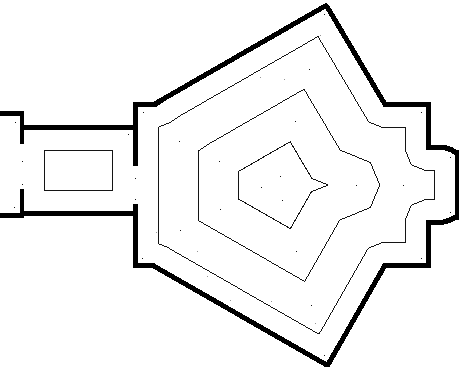
\includegraphics[width = \textwidth]{graphics/cup_collect_plan}
%     \caption{Part of the offline generated map for cup collection. The coordinates in \(S_{M}\) are marked.}
%     \label{cup_collect_plan}
%   \end{subfigure}
%   \begin{subfigure}[t]{0.3\textwidth}
%     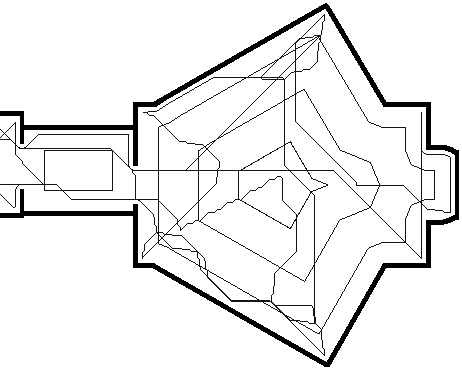
\includegraphics[width = \textwidth]{graphics/cup_collect_robot}
%     \caption{Part of the traveled path in cup collection. The coordinates visited are marked.}
%     \label{cup_collect_robot}
%   \end{subfigure}
% \caption{Cup collection planned vs. traveled}
% \label{cup_collection_results}
% \end{figure}